\documentclass[UTF8]{ctexart}
%前言部分
\usepackage{graphicx}%包含图片操作的包
\title{文章的标题}
\author{zjt}
\date{\today}
%正文部分
\begin{document}

\maketitle
\section{这是第一个章节}
你好!!!%一般输入
\textbf{加粗文字}
\textit{斜体},
\underline{下划线}
\section{这是第二个章节}
新的段落%两个回车表示新开一段,一个回车表示空格
\section{这是第三个章节}
\subsection{这是第一个子章节}
\subsubsection{这是第二个子章节}
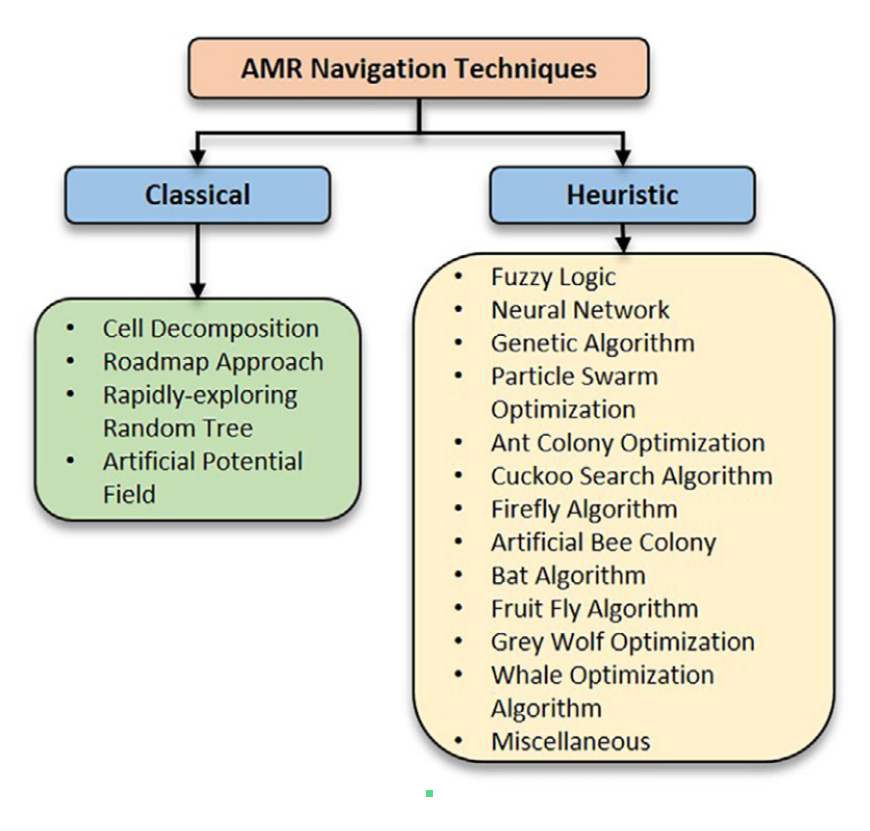
\includegraphics[width=0.5\textwidth]{image}%省去.pbg,尺寸0.5倍test宽度

\begin{figure}
\centering%图片居中
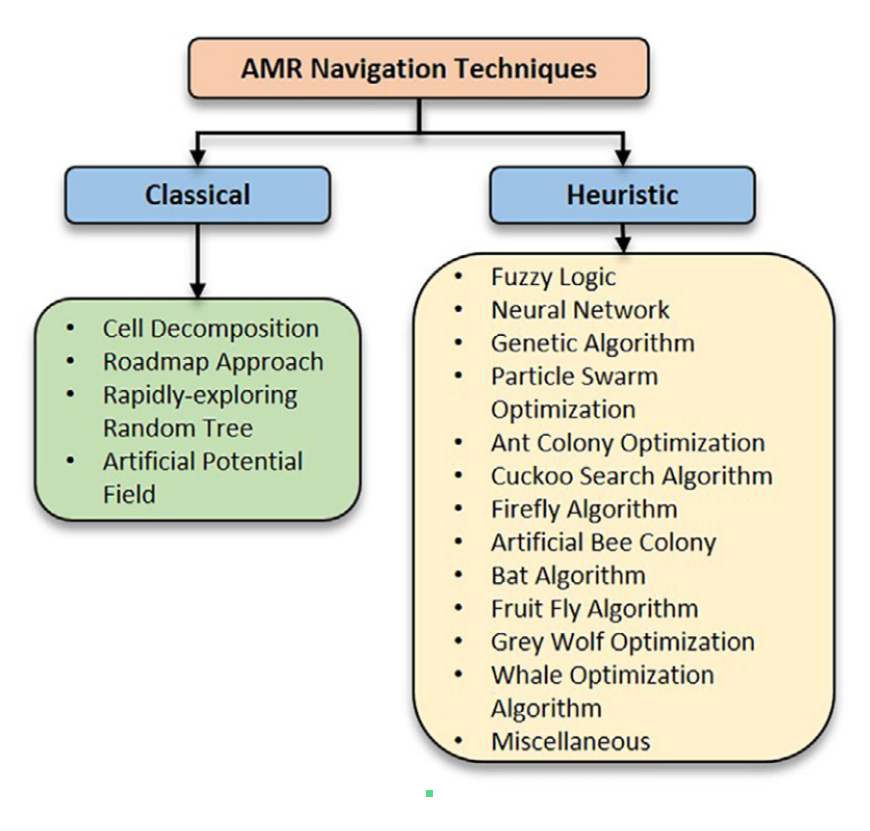
\includegraphics[width=0.5\textwidth]{image}
\caption{标题:这是一张图片}
\end{figure}


\begin{itemize}%无序列表
    \item 无序列表元素1
    \item 无序列表元素2
    \item 无序列表元素3
\end{itemize}

\begin{enumerate}
    \item 有序列表元素1
    \item 有序列表元素2
    \item 有序列表元素3
\end{enumerate}

存在方程:$E=mc^2$
\begin{equation}
    E=mc^2
\end{equation}%方程简写
\[
    E=mc^2
\]
\begin{tabular}{|l|c|r|p{2cm}|}%表示有四列,c为居中对齐,l为左对齐,r为右对齐,p为允许设置列宽,|表示元素元素间存在竖线
    \hline%水平线
    元素1 & 元素2 & 元素3 & 元素4 \\
    \hline\hline%双横线
    元素1 & 元素2 & 元素3 & 元素4 \\
    \hline
    元素1 & 元素2 & 元素3 & 元素4 \\
    \hline
\end{tabular}
\begin{table}%环境设置,可用于为表格添加标题
    \center
    \begin{tabular}{|l|c|r|p{2cm}|}%表示有四列,c为居中对齐,l为左对齐,r为右对齐,p为允许设置列宽,|表示元素元素间存在竖线
        \hline%水平线
        元素1 & 元素2 & 元素3 & 元素4 \\
        \hline\hline%双横线
        元素1 & 元素2 & 元素3 & 元素4 \\
        \hline
        元素1 & 元素2 & 元素3 & 元素4 \\
        \hline
    \end{tabular}
    \caption{标题:这是一个表格}
\end{table}
\end{document}